\documentclass{article}

% Language setting
% Replace `english' with e.g. `spanish' to change the document language
\usepackage[english]{babel}

% Set page size and margins
% Replace `letterpaper' with `a4paper' for UK/EU standard size
\usepackage[letterpaper,top=2cm,bottom=2cm,left=3cm,right=3cm,marginparwidth=1.75cm]{geometry}

% Useful packages
\usepackage{amsmath}
\usepackage{graphicx}
\usepackage[colorlinks=true, allcolors=blue]{hyperref}

\title{Panoramic Image Reconstruction}
\author{Charbel Abi Hana - \textit{charbel-a-h@outlook.com}}

\begin{document}
\maketitle

\section{Introduction}

The objective of this workshop is to construct a panoramic image out of two sequential images. We aim to reconstruct the panoramic image by using four corresponding points mapping the left and the right images. We will be using \href{http://imagine.enpc.fr/~monasse/Imagine++/index.html}{Imagine++} library for our code development. 

\section{Walk-through}
In the workshop files, we have two images labeled \textbf{image0006.txt} and \textbf{image0007.txt}. The images are shown below.
\begin{figure}%
    \centering
    {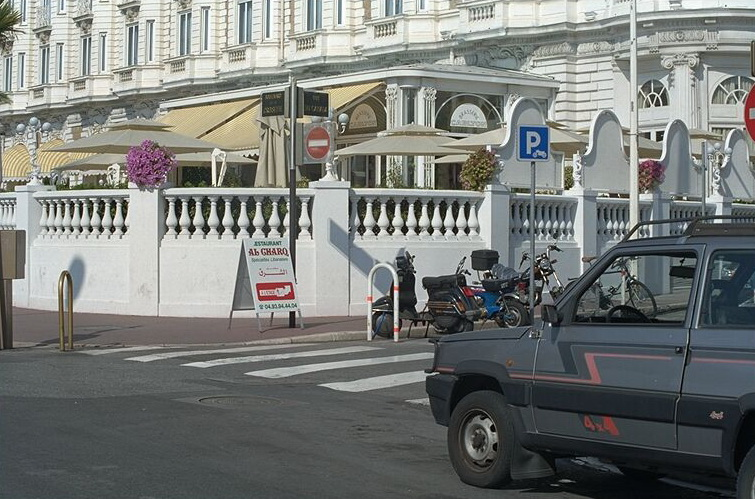
\includegraphics[width=7cm]{image0006.jpg} }%
    \qquad
    {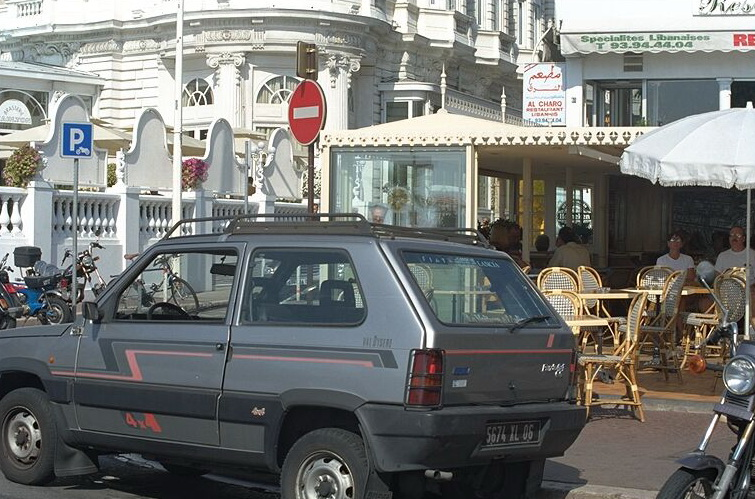
\includegraphics[width=7cm]{image0007.jpg} }%
    \caption{Left and Right images required for panoramic reconstruction}%
    \label{fig:example}%
\end{figure}

To reconstruct a panoramic image, we follow the steps below:
\begin{enumerate}
    \item Run cmake .
    \item Run make Panorama; ./Panorama
    \item Using the left mouse button, click on 4 or more points
    \item To finish the first points selection, press the right click button
    \item The second image will be set as current window. Follow the same step and select the  \textbf{corresponding} on the second image.
    \item Press right click to exit the points selection
\end{enumerate}
After completing these steps, the reconstructed panoramic image will be generated.

\section{Some Theoretical Background}
\subsection{Camera Calibration Matrix}
Following the pinhole camera model (single point aperture), we can derive the following equation for calculating the pixel coordinates of a projected 3D point:
\begin{equation}
    \textbf{x} = \begin{pmatrix} f & 0 & c_{x}\\ 0 & f & c_{y} \\ 0 & 0 & 1\end{pmatrix}\begin{pmatrix} R & T\end{pmatrix}\begin{pmatrix} X\\Y\\Z\\1\end{pmatrix}
\end{equation}
Where, the internal calibration matrix $\mathcal{K (3x3)}$ is defined as:
\begin{equation}
    K = \begin{pmatrix} f & 0 & c_{x}\\ 0 & f & c_{y} \\ 0 & 0 & 1\end{pmatrix}
\end{equation}
And the projection matrix $\mathcal{P (3x4)}$ is defined as:
\begin{equation}
    P = K \begin{pmatrix} R & T \end{pmatrix}
\end{equation}

\subsection{Homographies}
In homogeneous coordinates, the pixel values of the projection of the 3D points can also be expressed as:
\begin{equation}
    \begin{pmatrix} u \\ v \\ w \end{pmatrix} = \lambda\begin{pmatrix} C_{11} & C_{12} C_{13} & C_{14} \\ C_{21} & C_{22} C_{23} & C_{24} \\ C_{31} & C_{32} C_{33} & C_{34} \\ C_{41} & C_{42} C_{43} & C_{44} \\  \end{pmatrix} \begin{pmatrix}
    X \\ Y \\ Z \\ 1
    \end{pmatrix}
\end{equation}
With lambda being a scale factor. The result of scaling does not affect the equation in the homogeneous coordinates therefore we can replace $\mathcal{C_{44} = 1}$.
Considering 3D points on a plane, we can also reduce the projection matrix to:

\begin{equation}
    \begin{pmatrix} u \\ v \\ w \end{pmatrix} = \lambda\begin{pmatrix} C_{11} & C_{12}  & C_{14} \\ C_{21} & C_{22}  & C_{24} \\ C_{31} & C_{32}  & 1  \end{pmatrix} \begin{pmatrix}
    X \\ Y \\ 0 \\ 1
    \end{pmatrix}
\end{equation}

And we will write:
\begin{equation}
    \begin{pmatrix} u \\ v \\ w \end{pmatrix} = \lambda\begin{pmatrix} H_{11} & H_{12}  & H_{13} \\ H_{21} & H_{22}  & H_{23} \\ H_{31} & H_{32}  & 1  \end{pmatrix} \begin{pmatrix}
    X \\ Y \\ 1
    \end{pmatrix}
\end{equation}
Where the homography matrix $\mathcal{H (3x3)}$ is:
\begin{equation}
    H = \begin{pmatrix} H_{11} & H_{12}  & H_{13} \\ H_{21} & H_{22}  & H_{23} \\ H_{31} & H_{32}  & 1  \end{pmatrix}
\end{equation}
Once again the scale factor is arbitrary. There are 8 unique numbers in the homography matrix, therefore we can estimate each of those numbers by using 4 world points and their corresponding image points.
We can use this matrix to apply the following relation:
\begin{equation}
    \textbf{x'} = H\textbf{x}
\end{equation}
This equation transforms each pixel in our image through the homography matrix to obtain for example an un-distorted image as shown below in figure 2.

\begin{figure}%
    \centering
    {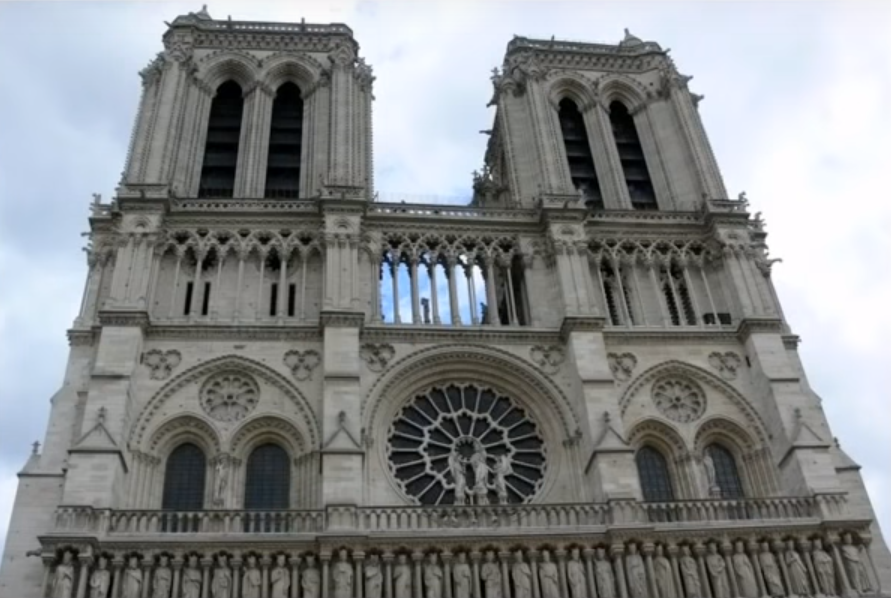
\includegraphics[width=7cm]{note_dame_distorted.png}}%
    \qquad
    {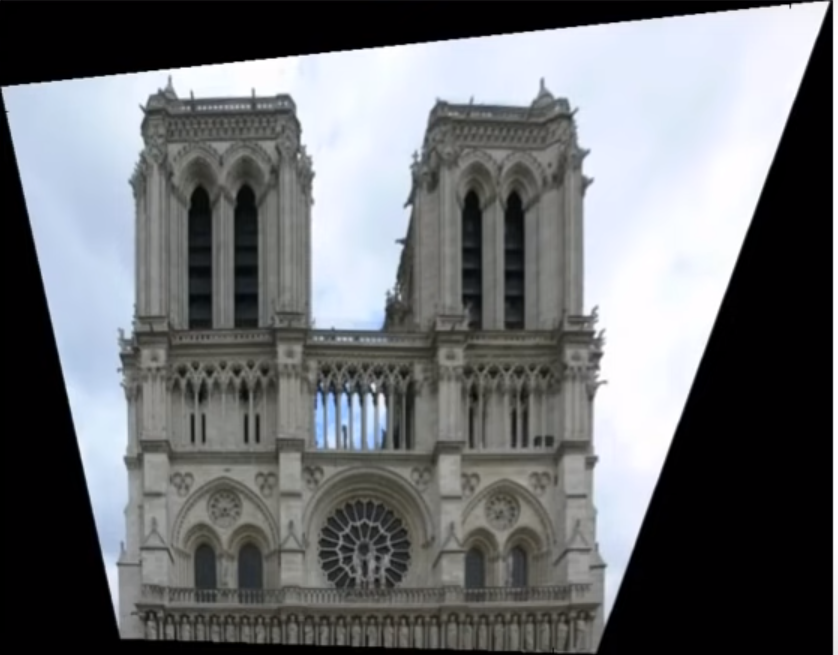
\includegraphics[width=6cm]{notre_dame_undistorted.png}}%
    \caption{(Right) distorted image of notre-dame, (left) undistorted image of note-dame}%
    \label{fig:example}%
\end{figure}

\subsection{Panoramic Construction}
In addition to distortion adjustment, we also use the homography matrix in panoramic reconstruction. We need to estimate a homography vector $\mathcal{H}$ of 9 rows; \begin{equation}
    h = \begin{pmatrix}
    H_{11} & H_{12} ... H_{33}
    \end{pmatrix}^T
\end{equation}
For each pair of corresponding points, we can write a matrix $\mathcal{A}$ which maps a point from the first image to its corresponding pair. By calculating the relation; \begin{equation}
    \textbf{x}_{i}' \times (H\textbf{x}_{i}) = 0
\end{equation}
\begin{equation}
    A_ih = 0
\end{equation}
With $\mathcal{A_i}$; 
\begin{equation}
    A_i = \begin{pmatrix}
    x_i & y_i & 1 & 0 & 0 & 0 & -x_i'x_i & -x_i'y_i \\
    0 & 0 & 0 & x_i & y_i & 1 & -y_i'x_i & -y_i'y_i
    \end{pmatrix}
\end{equation}

By solving the linear equations, we can estimate the homography matrix $\mathcal{H}$. Then we can use one of two methods to reconstruct the panoramic image; \textbf{pull} or \textbf{push}.
\begin{enumerate}
    \item \textbf{push} pixels to transformed image and round to the nearest pixel center. 
    \item \textbf{pull} pixels from original image by interpolation.
\end{enumerate}
We then can average pixel values at overlapping pixel positions to obtain the final reconstructed image.
\begin{figure}%
    \centering
    {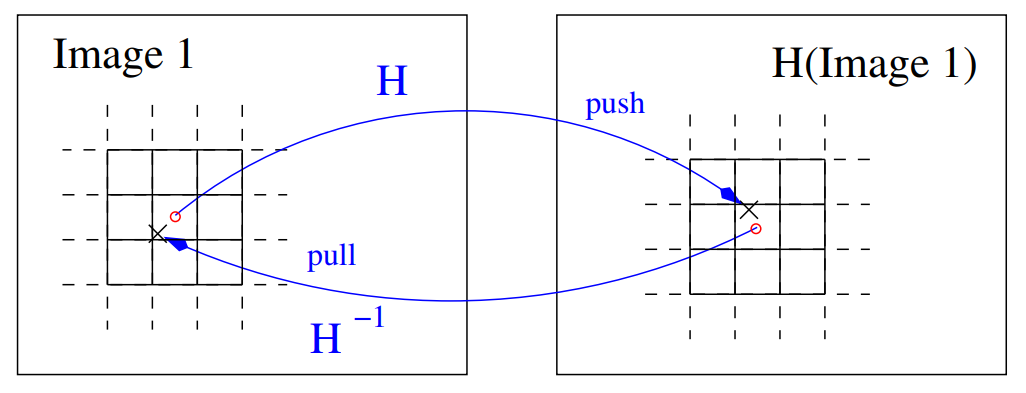
\includegraphics[width=10cm]{pull_push.png}}%
    \caption{Pull, Push methods for panoramic reconstruction, \href{http://imagine.enpc.fr/~monasse/Stereo/}{Source}}%
    \label{fig:example}%
\end{figure}

\subsection{Results}
In the workshop we reconstructed two images into one panoramic image. The points chosen in the step detailed earlier are shown in figure 4 below:
\begin{figure}%
    \centering
    {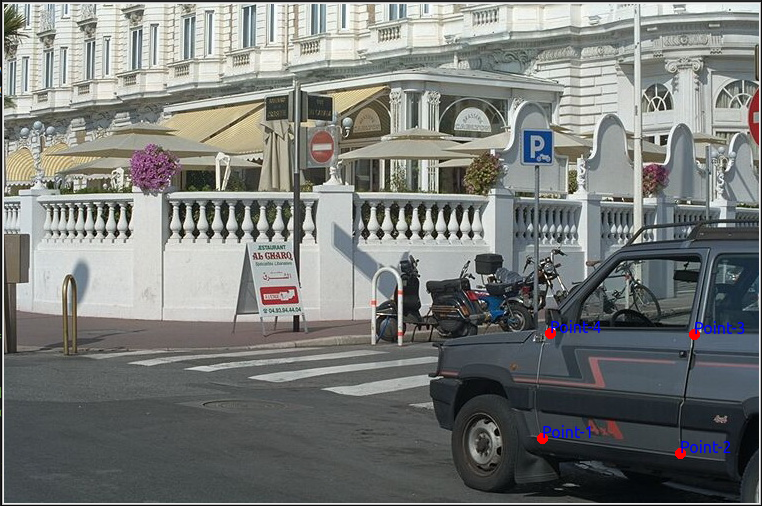
\includegraphics[width=10cm]{points.png}}%
    \caption{Matching points picked out of the first image}%
    \label{fig:example}%
\end{figure}

Applying corresponding points we obtain the following reconstructed image:
\begin{figure}%
    \centering
    {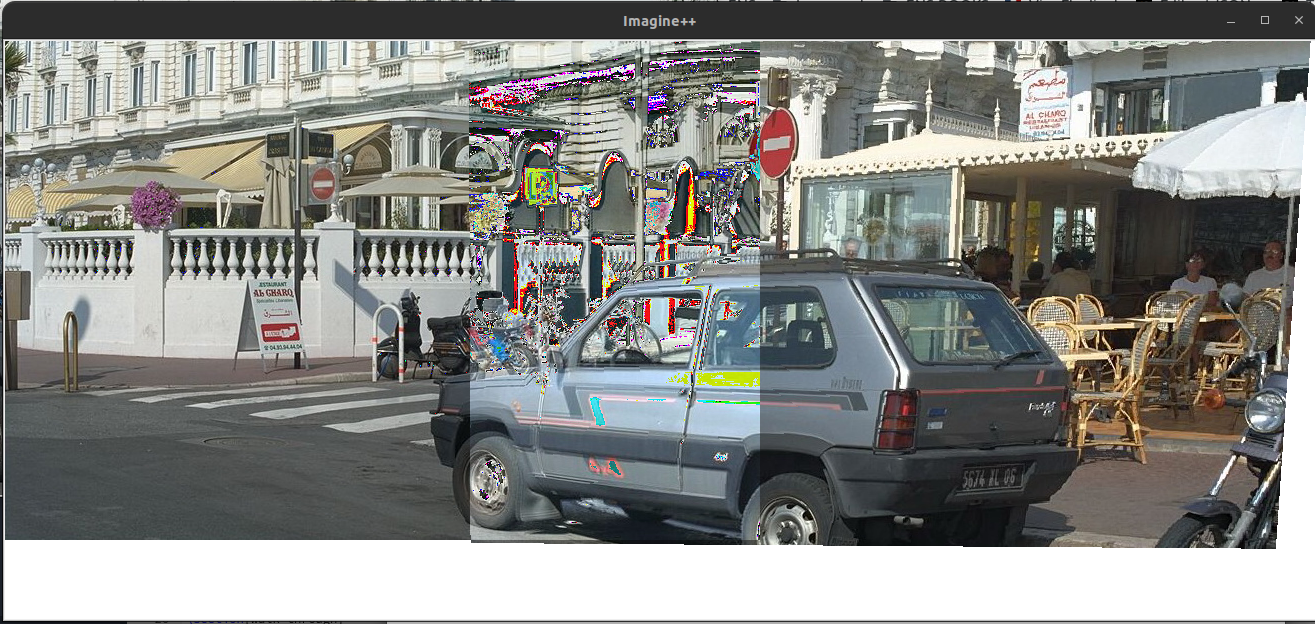
\includegraphics[width=15cm]{reconstructed.png}}%
    \caption{Reconstructed image}%
    \label{fig:example}%
\end{figure}
We observe some irregular colors, in the blending area of the panoramic reconstruction and we believe we can improve the quality of the obtained image by picking better and more representative points (more accurate choice of points and better suited to lie on planes), in addition, in overlaping areas we took the mean of the pixel values which also probably contributed to the different shades of color.
\end{document}